%!TEX root =  main.tex
\section{Introduction}


\begin{figure*}[ht!]
  \centering
  \begin{subfigure}[b]{0.45\textwidth}
    \centering
    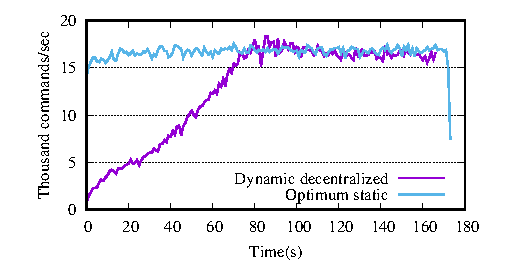
\includegraphics[width=0.95\columnwidth]{figures/motivation-tp-strong-locality}    
    \caption{Throughput with strong locality.}
  \end{subfigure}
  \begin{subfigure}[b]{0.45\textwidth}
    \centering
    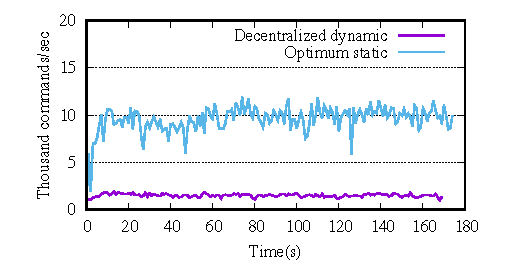
\includegraphics[width=0.95\columnwidth]{figures/motivation-tp-weak-locality}
    \caption{Throughput with weak locality}
  \end{subfigure} \\
  \begin{subfigure}[b]{0.45\textwidth}
    \centering
    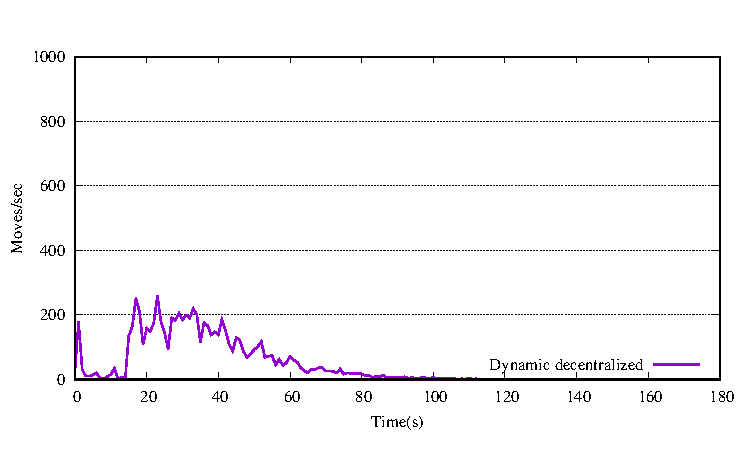
\includegraphics[width=0.95\columnwidth]{figures/motivation-moves-strong-locality}
    \caption{Number of move commands with strong locality.}
  \end{subfigure}
  \begin{subfigure}[b]{0.45\textwidth}
    \centering
    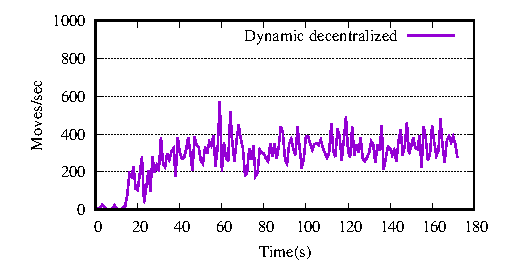
\includegraphics[width=0.95\columnwidth]{figures/motivation-moves-weak-locality}
    \caption{Number of move commands with weak locality}
  \end{subfigure} 
\end{figure*}




State machine replication (SMR) is a fundamental technique for
building fault tolerant systems and services. With SMR, state is
replicated on a set of servers, and each replica deterministically
executes the same sequence of client commands in order to maintain
consistency. Unfortunately, classic state machine replication does not
scale, since each replica must execute every command. In order to
improve the scalability of SMR, several systems have investigated the
use of state partitioning~\cite{facebookTAO, sciascia2012sdur,
  Aguilera:2007}.

In principle, increasing the number of partitions should result in
increased system performance. However, if executing a command
requires that the system access multiple partitions, then performance
can actually decrease, due to overhead from ordering commands across partitions to
ensure strong consistency. Moreover, if data is not distributed
carefully, then load imbalances can nullify the benefits of
partitioning.  Thus, an ideal partitioning scheme is one that would
both (i) minimize multiple partition commands, and (ii) provide load
balancing among the partitions. We refer to workloads that can be
partitioned in a way that satisfies these two properties as exhibiting
\emph{strong locality}.
\ef{i) and ii) don't imply our definition of strong locality}

Broadly speaking, there are two classes of techniques for
partitioning: \emph{static} and \emph{dynamic}.
Figure~\ref{fig:motivation} shows the result of a motivating experiment
that highlights the shortcomings of both of these approaches. In
the experiment, we show the throughput and number of state moves
over time with two different workloads; one with strong locality
and one with weak locality. For brevity, we postpone the details
of the experimental setup until Section~\ref{sec:experiments}.

Static schemes choose an immutable assignment of objects to partitions in
advance.  A prominent example of a
static scheme is S-SMR~\cite{bezerra2014ssmr}. One problem with static schemes is
that they cannot adapt as workloads change over time (e.g., in social
networks users join and leave the system, connections are created and
removed). One could imagine a static scheme that re-partitioned the
data based on every change in workload, but such a scheme would be
impossible to implement, since it would require a priori knowledge of
the workload. Figure~\ref{fig:motivation} shows the theoretical
optimal throughput one could achieve with a ``perfect'' static scheme.


Dynamic schemes are designed to address the problem with static
schemes.  Dynamic schemes assume no prior knowledge of the workload,
and move data to partitions on-demand in order to avoid
multi-partition commands. A prominent example of a dynamic scheme is
DS-SMR~\cite{hoang2016}. Unfortunately, existing dynamic schemes assume
workloads with strong locality. As Figure~\ref{fig:motivation} shows,
for workloads with weak-locality, DS-SMR suffers from instability due
to constantly moving data from one partition to another.


In this paper, we introduce \dynastar, a new approach to the state
partitioning problem designed to address these challenges.  \dynastar
is \emph{dynamic}. It does not require any a priori knowledge about
the workload, and it adapts to workload changes on-the-fly. However,
it is able to achieve throughputs comparable to the unrealizable
perfect static scheme. The key idea behind \dynastar is that it
minimizes the number of state relocations by monitoring the workload,
and re-computing an optimal partitioning on demand using a static
partitioner, we chose to use METIS partitioning algorithm~\cite{Abou-Rjeili:2006}
as an example of a static partitioner.
%ef.: Changed so we allow plug-and-play partitioners


With \dynastar, a location oracle maintains two data structures: (i) a
mapping of objects to partitions, and (ii) a \emph{workload graph}
with objects as vertices and edges as commands that access the
objects.  When a client submits a command, it must first contact the
location oracle to discover the partitions on which the objects are
stored.  If the command accesses objects in multiple partitions, the
oracle issues a move command to the partitions, re-locating objects to
a single partition. Of course, when re-locating an object, the oracle
is faced with a choice of which partition to use as a destination.
\dynastar chooses the optimal partition for relocation (i.e., one that
would minimize the number of state relocations) by partitioning the
workload graph using the METIS partitioner.




We have fully implemented \dynastar and compared its performance to
the dynamic partitioning protocol proposed by Long et
al.~\cite{hoang2016} and to the optimized static partitioning scheme.
Our prototype can handle workload graphs with half a million variables
and tens of millions of connections.  In workloads that present strong
locality, all three protocols eventually delivered comparable
performance, although \dynastar converged more quickly than the
decentralized scheme.  In workloads with weak locality, however,
\dynastar \emph{outperformed both} schemes.  The reason for the
surprisingly high performance of \dynastar compared to the optimized
static partitioning scheme is that \textbf{we need to explain this!!!
:-)} \ef{If the cost of migrating the object outperforms the cost of 
signaling partitions, why performance get similar when we have more partitions?} 
\lle{in static scheme, partitions exchange signal in every global commands,
while, in dynamic scheme, there is chance that partitions already have
data, thus no communication needed. More over, signaling is a two-way mechanism,
while moving objects in dynamic scheme is only one-way, which leads to less data
is being exchanged}

The paper makes the following contributions:
\begin{itemize}
\item It introduces \dynastar and discusses its implementation. 
\item It evaluates different partitioning schemes for state machine replication under a variety of conditions.
\item It describes \appname{} to demonstrate how \libname{} can be used to implement a scalable social network service.
\item It presents a detailed experimental evaluation of \dynastar including real social network graphs with half a million users and 14 million edges.
\end{itemize}

The rest of the paper is structured as follows.
Section~\ref{sec:sysmodel} describes our system model.
Section~\ref{sec:background} reviews existing scalable state machine replication approaches.
Section~\ref{sec:dssmr} introduces \dssmr{}; we explain the technique in detail and argue about its correctness.
Section~\ref{sec:implementation} details the implementation of \libname\ and \appname{}.
Section~\ref{sec:experiments} reports on the results of our experiments with \dssmr{}.
Section~\ref{sec:rw} surveys related work and
Section~\ref{sec:conclusion} concludes the paper.




%% %% Because single-partition commands are much more efficient than
%% %% multi-partition commands (i.e., in some cases by a factor of more than
%% %% 10x), the performance of a distributed storage system is particularly sensitive to the way
%% %% the service state is partitioned.


%% \subsection{State Machine Replication}

%% State machine replication (SMR) is a well-established technique to
%% develop highly available services (e.g.,
%% \cite{Shvachko:2003,Ghemawat:2003,Burrows:2006,MacCormick:2004}).  In
%% essence, the idea is that replicas deterministically execute the same
%% sequence of client commands in the same order and in doing so traverse
%% the same sequence of states and produce the same results.  State
%% machine replication provides configurable fault tolerance in the sense
%% that the system can be set to tolerate any number of faulty replicas.
%% Increasing the number of replicas, however, will not scale performance
%% since each replica must execute every command.  Unfortunately,
%% increasing the number of replicas will not scale performance since
%% each replica must execute every command.

%% S-SMR relies on an atomic multicast primitive to consistently order
%% commands within and across partitions.  Commands that access objects
%% located in a single partition (i.e., single-partition commands) are
%% multicast to the concerned partition and executed like in classical
%% SMR.  Commands that access objects located in multiple partitions
%% (i.e., multi-partition commands) are multicast to all involved
%% partitions.  To prevent command interleaves that violate strong
%% consistency, partitions coordinate during the execution of
%% multi-partition commands.



%% \subsection{Motivating Example}
